% Page 016 — page imprimée 12
% Suite de « ROMAN (Jean), vers 1668 - 1715 »
% Mise en page en deux colonnes.


{\fontsize{9.65}{11.05}\selectfont
\begin{multicols}{2}

la plupart s’enfuirent en Suisse, mais l’un fut rompu vif, d’autres moururent en prison. Ses blessures refermées, le prédicant reprit son apostolat, mais il était usé: il sortit définitivement du royaume en octobre 1699, guidé par Deleuze, de l’Espinas.

\section*{Dernières années en Suisse}

Arrivé à Lausanne, puis Berne, il se fit délivrer par divers pasteurs des attestations portant sur son ministère clandestin. A Rotterdam, sur les instances et grâce aux subsides des pasteurs, dont Jurieu, il publia sa \textit{Relation sommaire et véritable de ce que Dieu a fait par le ministère du Sr Jean Roman en quelques provinces de France, où il a prêché sous la croix pendant douze années} (1701, 89 p.), petit récit haut en couleurs des années de cendres et de braise qui suivirent 1685 en Cévennes; l’allusion de l’auteur à son ennemi, l’abbé du Chaila, resta la seule accusation portée par écrit avant l’assassinat du persécuteur, dont la nouvelle ferait le tour de l’Europe. Le synode wallon de Bois-le-Duc l’accueillit favorablement, et il obtint des Etats Généraux une pension de 400 livres pour un an, à charge d’aller desservir la communauté vaudoise de Waldensberg, près de Francfort. Roman, marié et père de famille depuis peu, rejoignit les vaudois, mais se heurta à leurs pasteurs, réunis en synode, qui refusèrent de le reconnaître comme l’un des leurs et de le consacrer, puisqu’il n’avait pas fait les études requises. Le conflit fut enfin dénoué au troisième synode vaudois (24 juin 1704, Francfort) : Roman fut consacré par les pasteurs Martel et Dautun (qu’il avait jadis rencontré en Cévennes); son ministère le conduisit à se transformer également en régent d’école; il reçut, défricha et cultiva lui-même 24 demi-arpents de terre, et resta à Waldensberg jusqu’à sa mort, ne laissant que deux enfants survivants sur les sept que son épouse, morte en 1713, lui avait donnés.

Il mourut à 47 ans, le 3 avril 1715, usé par ses douze années de clandestinité dans les hautes Cévennes. Ces dernières, depuis son départ, avaient connu le prophétisme, puis la guerre des Camisards, et s’apprêtaient à bénéficier du ministère d’une nouvelle génération de prédicants, autour d’Antoine Court et de Pierre Corteiz (*), ce dernier issu du quartier même que Roman avait si fidèlement parcouru.

\vspace{0.35em}

Bost (Ch.), Jean Roman. Prédicateur du Désert dans les Cévennes de 1687 à 1699, Neuilly, 1925, 30 p.; Les Prédicants protestants des Cévennes et du Bas-Languedoc, 1684-1700, Paris, 2 vol., 1912, passim.

\begin{flushright}
Patrick Cabanel\\[-0.1em]
« Lozériens connus ou à connaître »
\end{flushright}

\end{multicols}
}


\begin{center}
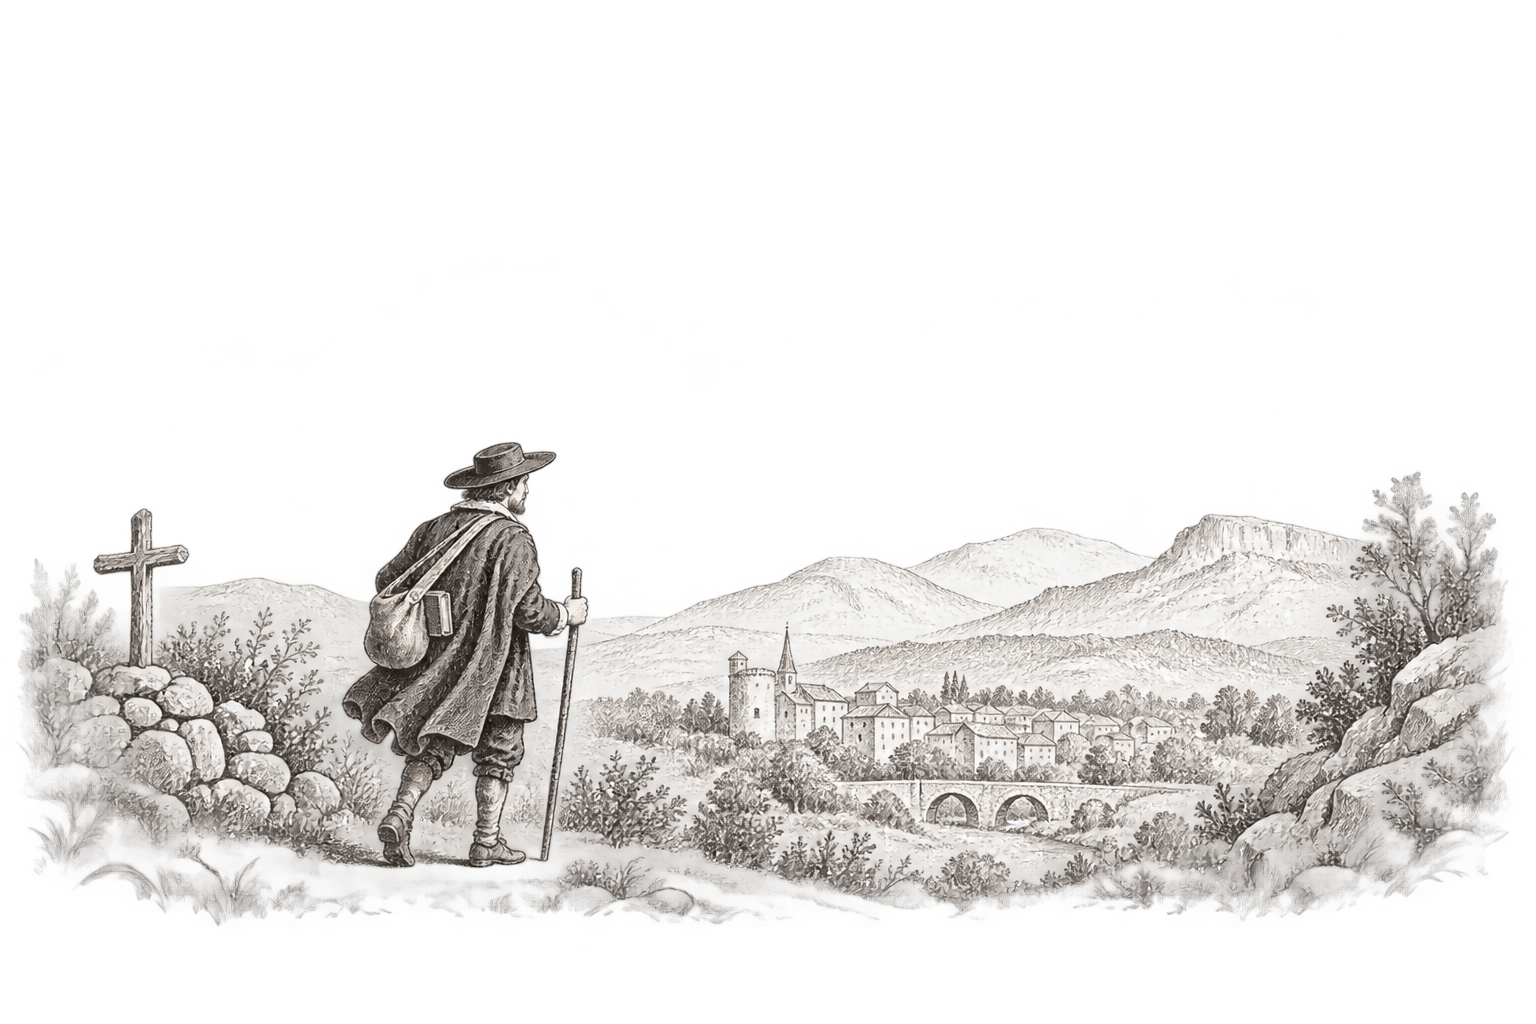
\includegraphics[width=\textwidth]{imgs/016.png}
\end{center}

